%*******************************************************************************
% Title: Ontoqa, Q&A with ontology-based natural language processing
%
% Conference: Courseworks in Artificial Intelligence
%
% Author: Antonella Botte <abotte@acm.org>
% Author: Giacomo Marciani <gmarciani@acm.org>
% Author: Debora Partigianoni <dpartigianoni@acm.org>
%
% Institution: Department of Civil Engineering and Computer Science Engineering,
%         University of Rome Tor Vergata, Italy
%
% Style: ACM Large VERSION 2017
%*******************************************************************************

\documentclass[acmlarge]{acmart}

%*******************************************************************************
% Packages
%*******************************************************************************
\usepackage[utf8]{inputenc}
\usepackage{amsmath}
\usepackage{booktabs}
\usepackage{lipsum}
\usepackage{caption}
\usepackage{array}
\usepackage{xr}
\usepackage{tikz}
\usepackage{tikz-qtree}
\usetikzlibrary{positioning}
\usepackage[ruled,noend,noline]{algorithm2e}

%*******************************************************************************
% Meta
%*******************************************************************************
\acmJournal{ACMROME-CP}
\acmVolume{1}
\acmNumber{1}
\acmArticle{1}
\acmYear{2017}
\acmMonth{2}
\acmArticleSeq{11}
\acmDOI{0000001.0000001}
\acmPrice{0.00}
\received[accepted]{February 2017}

%*******************************************************************************
% Copyright
%*******************************************************************************
\setcopyright{rightsretained}

%*******************************************************************************
% Algorithm
%*******************************************************************************
\usepackage[ruled]{algorithm2e}
\renewcommand{\algorithmcfname}{ALGORITHM}
\SetAlFnt{\small}
\SetAlCapFnt{\small}
\SetAlCapNameFnt{\small}
\SetAlCapHSkip{0pt}
\IncMargin{-\parindent}

%*******************************************************************************
% Custom Commands
%*******************************************************************************

%*******************************************************************************
% Numbering
%*******************************************************************************
\numberwithin{equation}{section}

%*******************************************************************************
% References
%*******************************************************************************
\externaldocument{sec/introduction}
\externaldocument{sec/background}
\externaldocument{sec/architecture}
\externaldocument{sec/grammar}
\externaldocument{sec/ontology}
\externaldocument{sec/parsing}
\externaldocument{sec/implementation}
\externaldocument{sec/sample-execution}
\externaldocument{sec/evaluation}
\externaldocument{sec/improvements}
\externaldocument{sec/conclusions}

\begin{document}
%*******************************************************************************
% Title and Authors
%*******************************************************************************
\title{Ontoqa, Q\&A with ontology-based natural language processing}
\author{Antonella Botte}
\orcid{0000-0000-0000-0000}
\affiliation{%
  \institution{University of Rome Tor Vergata}
  \streetaddress{Via del Politecnico 1}
  \city{Rome}
  \state{RM}
  \postcode{00133}
  \country{IT}}
\author{Giacomo Marciani}
\orcid{0000-0002-3675-8804}
\affiliation{%
  \institution{University of Rome Tor Vergata}
  \streetaddress{Via del Politecnico 1}
  \city{Rome}
  \state{RM}
  \postcode{00133}
  \country{IT}}
\author{Debora Partigianoni}
\orcid{0000-0000-0000-0000}
\affiliation{%
  \institution{University of Rome Tor Vergata}
  \streetaddress{Via del Politecnico 1}
  \city{Rome}
  \state{RM}
  \postcode{00133}
  \country{IT}}

%*******************************************************************************
% Front
%*******************************************************************************
\begin{abstract}
% GIACOMO
\lipsum[1]

\end{abstract}

% http://dl.acm.org/ccs.cfm

\begin{CCSXML}
	<ccs2012>
	<concept>
	<concept_id>10003752.10010124.10010138.10010145</concept_id>
	<concept_desc>Theory of computation~Parsing</concept_desc>
	<concept_significance>500</concept_significance>
	</concept>
	<concept>
	<concept_id>10010147.10010178.10010179.10010184</concept_id>
	<concept_desc>Computing methodologies~Lexical semantics</concept_desc>
	<concept_significance>500</concept_significance>
	</concept>
	<concept>
	<concept_id>10010147.10010178.10010179.10010186</concept_id>
	<concept_desc>Computing methodologies~Language resources</concept_desc>
	<concept_significance>500</concept_significance>
	</concept>
	<concept>
	<concept_id>10010147.10010178.10010187.10010195</concept_id>
	<concept_desc>Computing methodologies~Ontology engineering</concept_desc>
	<concept_significance>500</concept_significance>
	</concept>
	</ccs2012>
\end{CCSXML}

\ccsdesc[500]{Theory of computation~Parsing}
\ccsdesc[500]{Computing methodologies~Lexical semantics}
\ccsdesc[500]{Computing methodologies~Language resources}
\ccsdesc[500]{Computing methodologies~Ontology engineering}

\keywords{natural language processing; question answering; LTAG; DUDES}


%*******************************************************************************
% Thanks
%*******************************************************************************
\thanks{
  This work is supported by the Department of Civil Engineering and Computer Science
  Engineering, University of Rome Tor Vergata, Italy.\\
  Author's address:
  A. Botte, Via del Politecnico 1, Rome, RM 00133, Italy;
  email: abotte@acm.org;
  G. Marciani, Via del Politecnico 1, Rome, RM 00133, Italy;
  email: gmarciani@acm.org;
  D. Partigianoni, Via del Politecnico 1, Rome, RM 00133, Italy;
  email: dpartigianoni@acm.org;
}

\maketitle

\renewcommand{\shortauthors}{A. Botte, G. Marciani and D. Partigianoni}

%*******************************************************************************
% Core Content
%*******************************************************************************
\section{Introduction}
\label{sec:introduction}
% GIACOMO
\lipsum[1]

Lorem \cite{cimiano2014ontology}
\section{Background}
\label{sec:background}
% ANTONELLA
The context in which this work lies is the ontology-based interpretation of natural language. This approach puts ontology at the center of the interpretative process and assumes that for each ontology there are several lexicons, so this technique requires an expert to generate the specific lexicon for that ontology and domain.

Another aspect of this approach is the grammar used by the system for the interpretation of natural language in the context of a given ontology. These grammars are based on a vocabulary aligned with ontology and contain syntactic and semantic information that are crucial to the compositional process of the meaning of the sentence with respect to the precise ontology.
Domain-specific grammars are then used together with other domain-independent grammars, such as pronouns and auxiliary verbs.

%
This approach combines the ultimate purpose of the system realized as such tools will be used to build a question-answering system, where natural language application is transformed into a formal query through a linguistic analysis that is guided by the ontology grammar-based.
Formally, the three key aspects are defined:\textbf{Ontology}, \textbf{Grammar}, \textbf{Ontology Lexica}.

\subsection{Ontology}
\theoremstyle{definition}
\begin{definition}
\newtheorem{defn}{Definition}[section]{\textbf{Ontology}.Given a conceptualization \textit{C},an ontology \textit{O} is a logical theory with an ontological commitment  \textit{K} such that the models of the logical theory approximate as well as possible the set of intended models \begin{math}I_k(O)\end{math}}
\end{definition}

\subsection{Grammar}
The grammar consists of syntactic and semantic part:
\begin{itemize} 
  \item Syntax studies how words are combined into phrases and sentences
  \item Semantics investigates the meanings of expressions of a language, and how the meanings of basic expressions are combined into meanings of more complex expressions
\end{itemize} 
There are two particular formalisms for the representation of the semantics and syntax of a sentence.

%LTAG
The syntactic part is represented by LTAG( Lexicalized Tree Adjoining Grammar).  
The Tree Adjoining Grammar (TAG) is a linguistic formalism that builds on trees as representations of syntactic structure, and the TAG's fundamental hypothesis is that Every syntactic dependency is expressed locally within a single elementary tree. Lexicalized grammars assume that each atomic element or structure is associated with a lexical item. With respect to TAG, this means that elementary trees have to be associated with at least one lexical element, i.e., contain at least one leaf node labled with a non-empty terminal symbol, the anchor.

%DUDES
For semantic representation, we speak of representation DUDES (Dependency-based Underspecified Discourse REpresentation Structures.
A DUDES is a triple  \textit{(v,D,S)} where 
\begin{itemize} 
  \item  \textit{S} \begin{math}\epsilon \end{math} \textit{U} is a referent marker (the distinguished or main variable),
  \item \textit{D}=\textit{(U,C)} is a DRS with a discourse universe U and a set of conditions C, 
  \item  \textit{S} is a set of selection pairs of the form (N,v) where N is a LTAG tree node label and v is
a referent marker.
\end{itemize} 

\subsection{Ontology Lexica}
The Lexicon Model for Ontologies, or lemon for short, is such a model for specifying the lexicon-ontology interface, allowing one to state the meaning of lexical entries and constructions with respect to the vocabulary of a given ontology declaratively.

The lemon model follows a principle that has been referred to as semantics by referenceand states that the meaning of a lexical entry is specified by reference to a certain ontological class, property or individual.

The LexInfo ontology extends the lemon model with more than 600 specific linguistic categories.It can be used to add properties to different forms of a lexical entry. LexInfo is an ontology and thusallows for consistency checking and reasoning. 

In general, each lexical entry in a lemon lexicon has a number of syntactic arguments that map to semantic arguments of an ontological property or a more complex semantic frame. In general, we require that there is a one-to-one mapping between syntactic arguments subcategorized by a certain lexical entry and the set of semantic arguments specified in the lexical entry. For all lexical entries, we assume that there is a stereotypical usage or construction involving the lexical entry in which all syntactic arguments are actually realized.

%\section{Architecture}
\label{sec:architecture}
% ANTONELLA E DEBORA
\lipsum[1]
%\section{Grammar}
\label{sec:grammar}

% ANTONELLA E DEBORA
The LTAG/DUDES grammars consists of two parts: a domain-specific one obtained by extracting all relevant information from the ontology lexicon, and a domain-independent one created manually comprising closed-class expressions such as determiners, pronouns, copulative and auxiliary verbs.

It is important to note that the grammar entries are indexed with regular-expression, which represent the syntactic structure within the sentence. For this reason, the grammar entries can be composed not only by a single word but also by a more complex expression. The reader can refer to the Section~\ref{sec:parsing} for details on matching the specified entry in english natural language with the entries of LTAG/DUDES in the grammar.

\subsection{DOMAIN-SPECIFIC GRAMMAR}
Talking about the automatic generation of domain-specific grammar, we have created one LTAG/DUDES for each lexicon entry and for all its different forms. The types of lexicon entry we addressed are: \textit{verbs, common nouns, proper nouns, prepositions and adjectives}.

\subsubsection{VERBS}\mbox{}\\
All the verbs we need in the ontology lexicon in \textit{lemon} format are transitive verbs with active voice and indicative mood. The tree and the semantic representation would thus look as follows:

\medskip
\begin{center}
	\captionof{figure}{Grammar entry for: "acquire"}
\begin{tabular}{ p{10em} p{10em} }
	\label{tbl:grammar.acquire}
	
	\begin{center}
		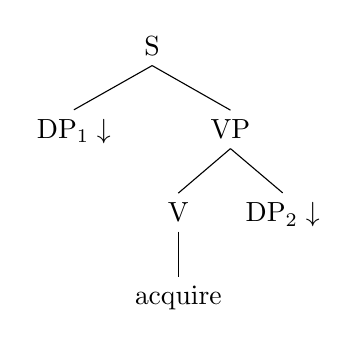
\begin{tikzpicture}
		\Tree [.S [.DP$_1\downarrow$ ] [.VP [.V acquire ] DP$_2\downarrow$ ] ]	
		\end{tikzpicture}
	\end{center}
	
	&

	\begin{center}
		\begin{tabular}{|c|l|}
			\hline
			\mbox{} & \mbox{}\\
			\hline
			\multicolumn{2}{|l|}{
				$isAcquiredBy(x,y)$
			} \\
			\hline
			\multicolumn{2}{|l|}{
				$(x,DP_{1}),(y,DP_{2})$
			} \\
			\hline
		\end{tabular}
	\end{center}	
	\\
\end{tabular}
\end{center}
\medskip

\subsubsection{NOUNS}\mbox{}\\
We can distinguish between common nouns, relational nouns and proper nouns. If the lexical entry of the ontology lexicon in \textit{lemon} has the tag \textit{possessiveAdjunct} we have a \textbf{relational noun} and the elementary LTAG/DUDES would thus look as follows: 

\medskip
\begin{center}
	\captionof{figure}{Grammar entry for: "chairman of"}
\begin{tabular}{ p{10em} p{10em} }
	\label{tbl:grammar.chairmanOf}
	
	\begin{center}
		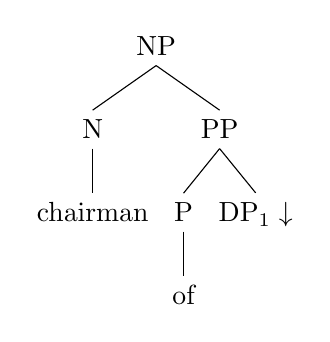
\begin{tikzpicture}
		\Tree [.NP [.N chairman ] [.PP [.P of ] DP$_1\downarrow$ ] ]
		\end{tikzpicture}
	\end{center}
		
	&
	
	\begin{center}
		\begin{tabular}{|c|l|}
			\hline
			y & \mbox{}\\ 
			\hline
			\multicolumn{2}{|l|}{
				$hasChairman(x,y)$
			} \\
			\hline
			\multicolumn{2}{|l|}{
				$(x,DP_{1})$
			} \\
			\hline
		\end{tabular}
	\end{center}	
	\\
\end{tabular}
\end{center}
\medskip

Simple common nouns and proper nouns differ from relational nouns in their syntactic behavior and sense. A \textbf{common noun}, as \textit{CEO, corporate officer}, and so on, has the following elementary LTAG/DUDES:

\medskip
\begin{center}
	\captionof{figure}{Grammar entry for: "people"}
\begin{tabular}{ p{10em} p{10em} }
	\label{tbl:grammar.people}
	
	\begin{center}
		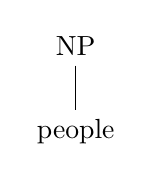
\begin{tikzpicture}
		\Tree [.NP people ]
		\end{tikzpicture}
	\end{center}
		
	&
	
	\begin{center}
		\begin{tabular}{|c|l|}
			\hline
			x & \mbox{}\\ 
			\hline
			\multicolumn{2}{|l|}{
				$Person(x)$
			} \\
			\hline
			\multicolumn{2}{|l|}{
				\mbox{}
			} \\
			\hline
		\end{tabular}
	\end{center}	
	\\
\end{tabular}
\end{center}
\medskip

A \textbf{proper noun}, e.g. \textit{Microsoft}, has instead the following elementary LTAG/DUDES:
 
\medskip
\begin{center}
	\captionof{figure}{Grammar entry for: "Microsoft"}
\begin{tabular}{ p{10em} p{10em} }
	\label{tbl:grammar.microsoft}
	
	\begin{center}
		
\begin{tikzpicture}
		\Tree [.DP Microsoft ]
		\end{tikzpicture}
	\end{center}
		
	&
	
	\begin{center}
		\begin{tabular}{|c|l|}
			\hline
			x & x\\ 
			\hline
			\multicolumn{2}{|l|}{
				$x=Microsoft$
			} \\

			\hline
			\multicolumn{2}{|l|}{
				\mbox{}
			} \\
			\hline
		\end{tabular}
	\end{center}	
	\\
\end{tabular}
\end{center}
\medskip

\subsubsection{ADJECTIVES}\mbox{}\\
We have different types of adjectives. Let's take some examples:
\begin{enumerate}
\item "\textit{an \textbf{italian} company}". In this case \textit{italian} is an \textbf{attributive} adjective and the associated grammar is the following:
 \medskip
\begin{center}
	\captionof{figure}{Grammar entry for: "italian" - attributive adjective}
\begin{tabular}{ p{10em} p{10em} p{10em} }
	\label{tbl:grammar.attributiveAdjective}
	
	\begin{center}
		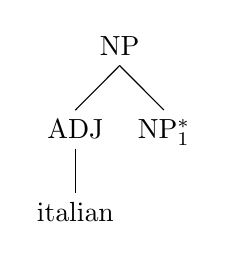
\begin{tikzpicture}
		\Tree [.NP [.ADJ italian ] [.NP$_1^\ast$ ] ]
		\end{tikzpicture}
	\end{center}
		
	&
	
	\begin{center}
		\begin{tabular}{|c|l|}
			\hline
			x & \mbox{}\\ 
			\hline
			\multicolumn{2}{|l|}{
				$hasNationality(x,y)$
			} \\
			\multicolumn{2}{|l|}{
				$y=Italy$
			} \\
			\hline
			\multicolumn{2}{|l|}{
				\mbox{}
			} \\
			\hline
		\end{tabular}
	\end{center}	
	
	&
	
	\begin{center}
		\begin{tabular}{|c|l|}
			\hline
			x & \mbox{}\\ 
			\hline
			\multicolumn{2}{|l|}{
				$hasHeadquarter(x,y)$
			} \\
			\multicolumn{2}{|l|}{
				$y=Italy$
			} \\
			\hline
			\multicolumn{2}{|l|}{
				\mbox{}
			} \\
			\hline
		\end{tabular}
	\end{center}	
	\\
\end{tabular}
\end{center}
\medskip
To note that \textit{italian} and similar adjectives are ambiguous in the lexicon. For more details on dealing with ambiguities, refer to Section~\ref{sec:parsing}.
\item "\textit{Is Satya Nadella \textbf{italian}?}". In this example \textit{italian} is a  \textbf{predicative} adjective and the elementary LTAG/DUDES are:
\medskip
\begin{center}
	\captionof{figure}{Grammar entry for: "italian" - predicative adjective}
\begin{tabular}{ p{10em} p{10em} p{10em}}
	\label{tbl:grammar.predicativeAdjective}
	
	\begin{center}
		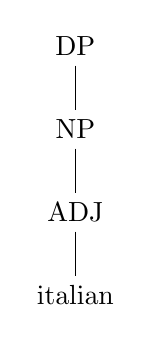
\begin{tikzpicture}
		\Tree [.DP  [.NP [.ADJ italian ] ] ]
		\end{tikzpicture}
	\end{center}
		
	&

	\begin{center}
		\begin{tabular}{|c|l|}
			\hline
			\mbox{x} & x y \\
			\hline
			\multicolumn{2}{|l|}{
				$hasNationality(x,y)$
			} \\
			\multicolumn{2}{|l|}{
				$y=Italy$
			} \\
			\hline
			\multicolumn{2}{|l|}{
				\mbox{}
			} \\
			\hline
		\end{tabular}
	\end{center}
	
	&
	
	\begin{center}
		\begin{tabular}{|c|l|}
			\hline
			\mbox{x} & x y \\
			\hline
			\multicolumn{2}{|l|}{
				$hasHeadquarter(x,y)$
			} \\
			\multicolumn{2}{|l|}{
				$y=Italy$
			} \\
			\hline
			\multicolumn{2}{|l|}{
				\mbox{}
			} \\
			\hline
		\end{tabular}
	\end{center}
	\end{tabular}
\end{center}
\medskip
\item "\textit{headquartered in Italy}". In this third case \textit{headquarters} is a \textbf{prepositional} adjective. The grammar is the following:

\medskip
\begin{center}
	\captionof{figure}{Grammar entry for: "headquartered in"}
\begin{tabular}{ p{10em} p{10em} }
	\label{tbl:grammar.headquarteredIn}
	
	\begin{center}
		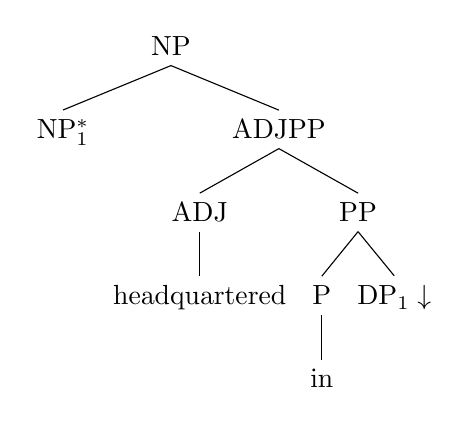
\begin{tikzpicture}
		\Tree [.NP [.NP$_1^\ast$ ] [.ADJPP [.ADJ headquartered ] [.PP [.P in ] DP$_1\downarrow$ ] ] ]	
		\end{tikzpicture}
	\end{center}
	
	&

	\begin{center}
		\begin{tabular}{|c|l|}
			\hline
			x & \mbox{}\\
			\hline
			\multicolumn{2}{|l|}{
				$hasHeadquarter(x,y)$
			} \\
			\hline
			\multicolumn{2}{|l|}{
				$(y,DP_{1})$
			} \\
			\hline
		\end{tabular}
	\end{center}	
	\\
\end{tabular}
\end{center}
\medskip
\item "\textit{Where is Microsoft headquartered?}". For adjectives as \textit{headquartered} the grammar contains a further entry composed by the regular expression "\textit{is * headquartered}". The "*" can represent any expression and this regular expression generates the following grammar:
\medskip
\begin{center}
	\captionof{figure}{Grammar entry for: "is * headquartered"}
\begin{tabular}{ p{10em} p{10em} }
	\label{tbl:grammar.is*headquartered}
	
	\begin{center}
		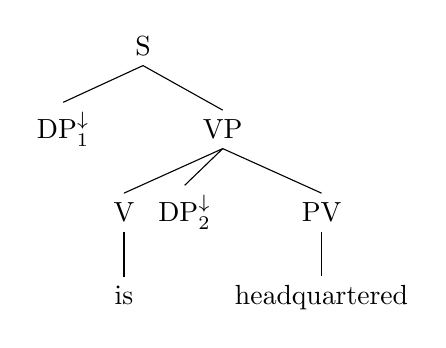
\begin{tikzpicture}
		\Tree [.S [.DP$_1^\downarrow$ ] [.VP [.V is ] DP$_2^\downarrow$ [.PV headquartered ] ] ]	
		\end{tikzpicture}
	\end{center}
	
	&

	\begin{center}
		\begin{tabular}{|c|l|}
			\hline
			\mbox{} & \mbox{}\\
			\hline
			\multicolumn{2}{|l|}{
				$hasHeadquarter(x,y)$
			} \\
			\hline
			\multicolumn{2}{|l|}{
				$(x, DP_{2}),(y,DP_{1})$
			} \\
			\hline
		\end{tabular}
	\end{center}	
	\\
\end{tabular}
\end{center}
\medskip
\end{enumerate}


\subsection{DOMAIN-INDEPENDENT GRAMMAR}
For the domain-independent expressions, we generate manually a fixed grammar entry for each word or expression we could encounter. For example there is a grammar for the expression \textit{how many}:
 \medskip
\begin{center}
	\captionof{figure}{Grammar entry for: "How many"}
\begin{tabular}{ p{10em} p{10em} }
	\label{tbl:grammar.howMany}
	
	\begin{center}
		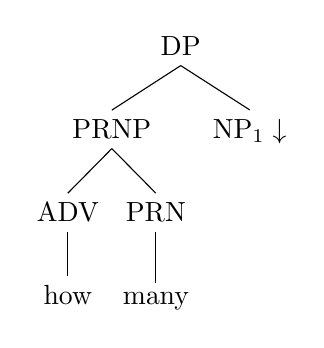
\begin{tikzpicture}
		\Tree [.DP  [.PRNP [.ADV how ] [.PRN many ]] [.NP$_1\downarrow$ ]]
		\end{tikzpicture}
	\end{center}
		
	&
	
	\begin{center}
		\begin{tabular}{|c|l|}
			\hline
			x & x\\ 
			\hline
			\multicolumn{2}{|l|}{
				$count(x)$
			} \\
			\hline
			\multicolumn{2}{|l|}{
				$(x,NP_{1})$
			} \\
			\hline
		\end{tabular}
	\end{center}	
	\\
\end{tabular}
\end{center}
\medskip

The auxiliary verbs, as \textit{do, does, did, have, has, had}, don't have a semantic interpretation, so the DUDES is empty. The elementary LTAG instead is in the form of adjunction tree:
\medskip
\begin{center}
	\captionof{figure}{Grammar entry for: "do"}
\begin{tabular}{ p{10em} p{10em} }
	\label{tbl:grammar.do}
	
	\begin{center}
		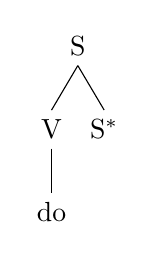
\begin{tikzpicture}
		\Tree [.S  [.V do ] [.S$^\ast$ ]]
		\end{tikzpicture}
	\end{center}
	&
	\begin{center}
		\begin{tabular}{|c|l|}
			\hline
			\mbox{} & \mbox{}\\ 
			\hline
			\multicolumn{2}{|l|}{
				\mbox{}
			} \\
			\hline
			\multicolumn{2}{|l|}{
				\mbox{}
			} \\
			\hline
		\end{tabular}
	\end{center}	
	\\
\end{tabular}
\end{center}
\medskip

We have generated grammar also for determiners, pronouns and copulative verbs. Determiners, i.e. \textit{the, a, an} has the following elementary LTAG/DUDES:
\medskip
\begin{center}
	\captionof{figure}{Grammar entry for: "the"}
\begin{tabular}{ p{10em} p{10em} }
	\label{tbl:grammar.the}
	
	\begin{center}
		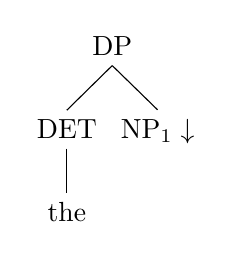
\begin{tikzpicture}
		\Tree [.DP  [.DET the ] [.NP$_1\downarrow$ ]]
		\end{tikzpicture}
	\end{center}
		
	&

	\begin{center}
		\begin{tabular}{|c|l|}
			\hline
			x & x\\ 
			\hline
			\multicolumn{2}{|l|}{
				\mbox{}
			} \\
			\hline
			\multicolumn{2}{|l|}{
				$(x,NP_{1})$
			} \\
			\hline
		\end{tabular}
	\end{center}	
	\\
\end{tabular}
\end{center}
\medskip

The grammar of wh-pronoun, as \textit{who, what, where, which}, is:
\medskip
\begin{center}
	\captionof{figure}{Grammar entry for: "who"}
\begin{tabular}{ p{10em} p{10em} }
	\label{tbl:grammar.who}
	
	\begin{center}
		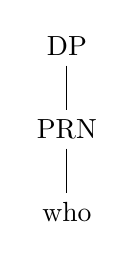
\begin{tikzpicture}
		\Tree [.DP  [.PRN who ] ]
		\end{tikzpicture}
	\end{center}
		
	&

	\begin{center}
		\begin{tabular}{|c|l|}
			\hline
			x & ?x\\ 
			\hline
			\multicolumn{2}{|l|}{
				\mbox{}
			} \\
			\hline
			\multicolumn{2}{|l|}{
				\mbox{}
			} \\
			\hline
		\end{tabular}
	\end{center}	
	\\
\end{tabular}
\end{center}
\medskip

Finally, we have to considered the copulative verbs. They have two different syntactic representations, for example consider the following questions:
\begin{enumerate}
\item \textit{Where is Microsoft headquartered?}
\item \textit{Is Satya Nadella the CEO of Microsoft?}
\end{enumerate}
In the first case, the copulative verb \textit{is} has the grammar :
\medskip
\begin{center}
	\captionof{figure}{Grammar entry for: "is" (1)}
\begin{tabular}{ p{10em} p{10em} }
	\label{tbl:grammar.is}
	
	\begin{center}
		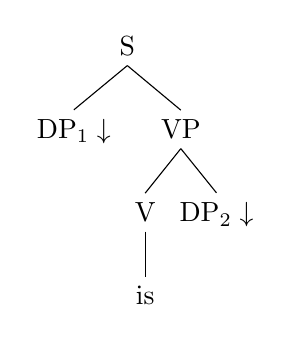
\begin{tikzpicture}
		\Tree [.S [.DP$_1\downarrow$ ] [.VP [.V is ] DP$_2\downarrow$ ] ]	
		\end{tikzpicture}
	\end{center}
	
	&

	\begin{center}
		\begin{tabular}{|c|l|}
			\hline
			\mbox{} & \mbox{}\\
			\hline
			\multicolumn{2}{|l|}{
				$replace(y,x)$
			} \\
			\hline
			\multicolumn{2}{|l|}{
				$(x,DP_{1}),(y,DP_{2})$
			} \\
			\hline
		\end{tabular}
	\end{center}	
	\\
\end{tabular}
\end{center}
\medskip

In the second case the grammar have to be the following:
\medskip
\begin{center}
	\captionof{figure}{Grammar entry for: "is" (2)}
\begin{tabular}{ p{10em} p{10em} }
	\label{tbl:grammar.is}
	
	\begin{center}
		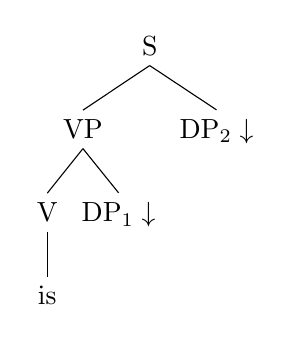
\begin{tikzpicture}
		\Tree [.S [.VP [.V is ] DP$_1\downarrow$ ] [.DP$_2\downarrow$ ] ]	
		\end{tikzpicture}
	\end{center}
	
	&

	\begin{center}
		\begin{tabular}{|c|l|}
			\hline
			\mbox{} & \mbox{}\\
			\hline
			\multicolumn{2}{|l|}{
				$replace(y,x)$
			} \\
			\hline
			\multicolumn{2}{|l|}{
				$(x,DP_{1}),(y,DP_{2})$
			} \\
			\hline
		\end{tabular}
	\end{center}	
	\\
\end{tabular}
\end{center}
\medskip
%\section{Ontology}
\label{sec:ontology}
% DEBORA
The domain chosen for our ontology is "Organizations". It has been created to answer the provided questions but it is not strongly restricted to them. A domain ontology expresses the links between specific objects and events of that domain through classes (or concepts), properties and attributes of the classes, constraints and instances.
The concepts we want to represent are:
\begin{itemize}
\item The companies.
\item People who play an important role in the company.
\item A nation for people or for the headquarter of a company.
\end{itemize}
The symbols we used to represent this sets are: \textit{Company, Person} and \textit{Nation}.
Then we need symbols to represent the relationships between classes. The relationships we needed are:
\begin{itemize}
\item A person who is the founder of a company.
\item A person who is the CEO of a company.
\item A person who is the CFO of a company.
\item A person who is the Chairman of a company.
\item A person who is the Corporate Officer of a company.
\item A company acquiring a company.
\item The nationality of people.
\item The nation where the headquarter of a company is located.
\end{itemize}
The symbols we used to represent these relationships are: \textit{hasFounder, hasCEO, hasCFO, hasChairman, hasCorporateOfficer, isAcquiredBy, hasNationality} and \textit{hasHeadquarter}. 
The last two are sub-properties of \textit{hasNation} property to solve the ambiguity in deciding if a nationality, for example \textit{italian}, refers to people or companies. Let's look at that in detail:
\begin{itemize}
\item \textit{hasNation} has \textit{"Person \textbf{or} Company"} as domain and \textit{Nation} as range.
\item \textit{hasHeadquarter} has \textit{Company} as domain and \textit{Nation} as range.
\item \textit{hasNationality} has \textit{Person} as domain and \textit{Nation} as range.
\item \textit{Person} is disjoint with \textit{Company}.
\end{itemize}

We also introduced some attribute to classes:
\begin{itemize}
\item The net income of an organization.
\item The market value of a company. For multinational company the market value is referred to the market capitalization. For smaller companies, subsidiaries whose business operations and investments are controlled by the parent corporation, the market value is referred to value at which a company is acquired.
\end{itemize}
The symbols we used to represent these attributes are: \textit{ netIncome} and \textit{marketValue}.
Both the net income and the purchase price are in \textit{billion U.S. dollars}. To note that a billion, in American English, has always equated to a thousand million (i.e. 1'000'000'000).

In order to prevent a computer program to use the symbols '\textit{in the wrong way}' we have introduced  constraints on the way the vocabulary is used:
\begin{itemize}
\item As already mentioned, a person can not be a company and a company can not be a person.
\item People must have at least one nationality. (????????solo una la nazionalità se intesa come nazione di nascita???????)
\item Companies must have at least one headquarter. 
\end{itemize}

The reader can refer to the two file \textit{organizationNotImportedInfer.ttl} and \text
The reader can refer to the files \textit{organization.ttl} and\textit{organizationNotImportedInfer.ttl} in the \textit{data/knowledge} package to see the ontology in detail. The first file is obtained merging the inferred and asserted information of our ontology. The second one contains only the asserted informations.  

Below an entity-relationship model (ER model) for our specific domain of knowledge.
\begin{figure}
\centering
\includegraphics[width=10cm, height=8cm]{ERDiagram.png}
\end{figure}


\section{Parsing}
\label{sec:parsing}
% GIACOMO

The parsing process is responsible to generate a DUDES from a question expressed in natural language. 
%
To achieve this, it takes in input a \textit{SLTAG grammar} and a \textit{question} expresed in english natural language.
The output of the parsing process is a \textit{DUDES} representing the semantic of the question.
%
The produced DUDES will then be used to generate a \textit{SPARQL query}, that can be submitted to the ontology which the SLTAG grammar is aligned to.
%

\begin{algorithm}[t]
\SetKwProg{Fn}{Function}{}{}  

\Fn{receive (x,y,w)} {
	
	\If{$(x,y)\in E(G)$}{
		updateLink(x,y,w) \\
		$U \leftarrow update(x) \cup update(y)$ \\
		\For{$u\in U$}{
			emitHidden(u)\;
		}
	}
	
	\ElseIf{$x\in V(G) \land y\in V(G)$}{
		addLink(x,y,w) \\
		$U \leftarrow update(x) \cup update(y)$ \\
		\For{$u\in U$}{
			emitHidden(u)\;
			emitPotential(u)\;
		}
	}
	
	\ElseIf{$x\in V(G) \land y\notin V(G)$}{
		addLink(x,y,w) \\
		$U \leftarrow update(y)$ \\
		\For{$u\in U$}{
			emitHidden(u)\;
			emitPotential(u)\;
		}
	}
	
	\ElseIf{$x\notin V(G) \land y\in V(G)$}{
		addLink(x,y,w) \\
		$U \leftarrow update(x)$ \\
		\For{$u\in U$}{
			emitHidden(u)\;
			emitPotential(u)\;
		}
	}  
	
	\Else{
		addLink(x,y,w)
	}
}

\Fn{update (x)}{
	$N \leftarrow Neighbors(x)$ \\
	$U \leftarrow \emptyset$ \\
	\For{$y\in N$}{
		\If{$(x,y)\notin E(G)$}{
			$U \leftarrow U \cup \{(x,y)\}$
		}
	}
	\For{$z\in N$}{
		\If{$(x,z)\notin E(G) \land z\neq y$}{
			$U \leftarrow U \cup \{(y,z)\}$
		}
	}
	\KwResult{$U$}
}
\caption{Parsing algorithm}
\label{alg:parsing}
\end{algorithm}

Some functions in Algorithm~\ref{alg:parsing} have not been formally defined because they are pretty self-explanatory. 
For reader's sake, we briefly describe them here. \texttt{emitHidden(u)} and \texttt{emitPotential(u)} let the operator emit tuples in the form \texttt{(x,y,HIDDEN)} and \texttt{(x,y,POTENTIAL)}, meaning that an hidden or potential score update is necessary for the edge $(x,y)$, respectively.
\texttt{updateLink(x,y,w)} updates the existent edge $(x,y)$ with the new EWMA weight value. 
\texttt{addLink(x,y,w)} inserts the edge $(x,y)$ with weight $w$. 
\texttt{Neighbors(x)} return the set of neighbors of $x$.

\begin{algorithm}[t]
	\SetKwProg{Fn}{Function}{}{}  
	
	\Fn{receive (x,y,w)} {
		
		\If{$(x,y)\in E(G)$}{
			updateLink(x,y,w) \\
			$U \leftarrow update(x) \cup update(y)$ \\
			\For{$u\in U$}{
				emitHidden(u)\;
			}
		}
		
		\ElseIf{$x\in V(G) \land y\in V(G)$}{
			addLink(x,y,w) \\
			$U \leftarrow update(x) \cup update(y)$ \\
			\For{$u\in U$}{
				emitHidden(u)\;
				emitPotential(u)\;
			}
		}
		
		\ElseIf{$x\in V(G) \land y\notin V(G)$}{
			addLink(x,y,w) \\
			$U \leftarrow update(y)$ \\
			\For{$u\in U$}{
				emitHidden(u)\;
				emitPotential(u)\;
			}
		}
		
		\ElseIf{$x\notin V(G) \land y\in V(G)$}{
			addLink(x,y,w) \\
			$U \leftarrow update(x)$ \\
			\For{$u\in U$}{
				emitHidden(u)\;
				emitPotential(u)\;
			}
		}  
		
		\Else{
			addLink(x,y,w)
		}
	}
	
	\Fn{update (x)}{
		$N \leftarrow Neighbors(x)$ \\
		$U \leftarrow \emptyset$ \\
		\For{$y\in N$}{
			\If{$(x,y)\notin E(G)$}{
				$U \leftarrow U \cup \{(x,y)\}$
			}
		}
		\For{$z\in N$}{
			\If{$(x,z)\notin E(G) \land z\neq y$}{
				$U \leftarrow U \cup \{(y,z)\}$
			}
		}
		\KwResult{$U$}
	}
	\caption{Tokenization algorithm}
	\label{alg:tokenization}
\end{algorithm}

Some functions in Algorithm~\ref{alg:tokenization} have not been formally defined because they are pretty self-explanatory. 
For reader's sake, we briefly describe them here. \texttt{emitHidden(u)} and \texttt{emitPotential(u)} let the operator emit tuples in the form \texttt{(x,y,HIDDEN)} and \texttt{(x,y,POTENTIAL)}, meaning that an hidden or potential score update is necessary for the edge $(x,y)$, respectively.
\texttt{updateLink(x,y,w)} updates the existent edge $(x,y)$ with the new EWMA weight value. 
\texttt{addLink(x,y,w)} inserts the edge $(x,y)$ with weight $w$. 
\texttt{Neighbors(x)} return the set of neighbors of $x$.
\section{Implementation}
\label{sec:implementation}
% ALL
\lipsum[1]
%\section{Sample execution}
\label{sec:sample-execution}
% DEBORA
\lipsum[1]
\section{Evaluation}
\label{sec:evaluation}
We evaluate the performance of our solution on a single general purpose
Amazon EC2 m3.large instance, running Debian 8.3 (Jessie)
and equipped with an Intel Xeon E5-2670 v2 (Ivy Bridge)  (2.6 GHz,
8 cores and 20 MB cache), 7.5 GB of RAM and a general purpose SSD.
%
The experimental framework consists in evaluating the performance achieved by Ontoqa in terms of response-time.
%
The input considered in experimentations are questions characterized by distinct complexities, in terms of structure and ambiguities.

\begin{figure}[H]
	\centering
	\includegraphics[width=0.8\columnwidth]{./fig/evaluation-response-time}
	\caption{Response time performance of Ontoqa on the benchmark questions.}
	\label{fig:evaluation-response-time}
\end{figure}

In particular we examine the following class of questions:

\begin{itemize}
	\item[Q1] questions in the form \textit{'who founded Microsoft?'}.
	\item[Q2] questions in the form \textit{'who are the corporate officers of Microsoft?'}.
	\item[Q3] questions in the form \textit{'where is Microsoft headquartered?'}.
	\item[Q4] questions in the form \textit{'what is the most valuable company?'}.
	\item[Q5] questions in the form \textit{'who are the corporate officers of the most valuable company?'}.
	\item[Q6] questions in the form \textit{'is Satya Nadella the CEO of Microsoft?'}.
	\item[Q7] questions in the form \textit{'did Microsoft acquire a company headquartered in Italy?'}.
	\item[Q8] questions in the form \textit{'is Satya Nadella italian?'}.
	\item[Q9] questions in the form \textit{'did Microsoft acquire an italian company?'}.
\end{itemize}

Notice that questions \texttt{Q1-Q7} do not induce any semantic ambiguity, while questions \texttt{Q8} and \texttt{Q9} do due to the presence of the entry \textit{'italian'}. In fact, the latter can be referred both to companies (e.g. a company headquartered in Italy) and to people (e.g. a person with italian nationality).
%
The experiments have been carried out by averaging measurements on randomly ordered 10 executions.
%
Figure~\ref{fig:evaluation-response-time} shows, the \textit{response time} achieved by Ontoqa when facing with the benchmark questions \texttt{Q1}-\texttt{Q8}.
%
The former has been measured considering the time elapsed for the question to be answered, calling the Java built-in function \texttt{System.currentTimeMillis()}.

The results are coherent with the theoretical and implementation framework. In fact, we can observe that (i) unambiguous questions (\texttt{Q1-Q7}) induce a response time proportional to the depth of the generated LTAG and (ii) the questions involving ambiguities (\texttt{Q8 and Q9}) induce a response time proportional to the complexity of the ambiguity.
\section{Further Improvements}
\label{sec:improvements}

\lipsum[1]
\section{Conclusions}
\label{sec:conclusions}

In this work we described Ontoqa, a Q\&A web and standalone application which aims to adapt easily to distinct ontologies and lexicons.
%
The proposed solution leverages ontology-driven NLP through the use of the LTAG/DUDES model and a greedy parsing algorithm aiming to reduce both the syntactic and semantic search space.
%
%
% RESULTS
The experimental results show that our system can answer the benchmark questions, with good performance with respect to both response-time and memory usage. 
%
%
% CONCLUSIONS
Our work shows that ontology alignment through the LTAG/DUDES model permits 
high modularization and generalization of the NLP process.
%
Furthermore, such a model suits well to the design of parsing algorithms that can effectively minimize both the syntactic and semantic search space.


%*******************************************************************************
% Bibliography
%*******************************************************************************
\bibliographystyle{acmreferences}
\bibliography{ref/biblio}

\end{document}
